\section{1.1}

\textit{Hvad kan i lave med 10 blokke?}

Ved hjælp af disse 10 blokke vil vi lave et ‘sjovt program’.

\begin{figure}[ht]
	\centering
	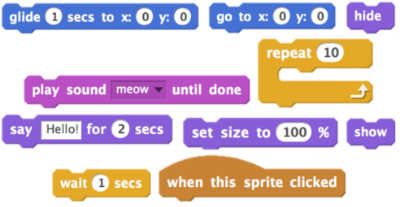
\includegraphics[scale=0.8]{10_ScratchBloks.png}
	\caption{{10 Scratch Bloks}}
	\label{fig:10Bloks}
\end{figure}

Den eneste programmet kan lytte på, er om en sprite klikkes eller ej.

\subsection{Version 0.1:}

Hypotese:

\begin{figure}[ht]
	\centering
	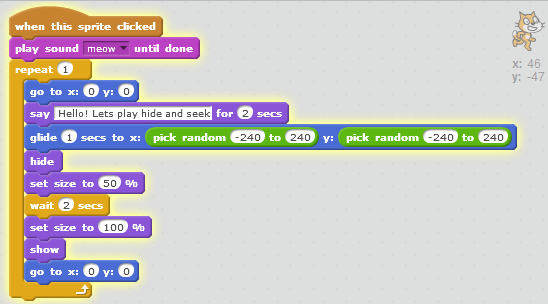
\includegraphics[scale=0.8]{10_ScratchBloks_Version01.png}
	\caption{{10 Scratch Bloks}}
	\label{fig:Version_0.1}
\end{figure}

\begin{itemize}
	\item Når vi klikker på vores sprite vil den begynde at miave.
	\item Gå til sin startposition og sige Let’s play hide and seek.
	\item Bevæge sig til et tilfældigt x,y koordinat mellem minus 240 og 240.	
	\item Så skjules spriten og den halveres i størrelse.
	\item Scriptet venter i 2 sekunder.
	\item Genskaber original størrelse (Trinnet er inkluderet for at bruge størrelses-commands).
	\item Spriten dukker op på det koordinat hvor den gemte sig.
	\item Spriten går tilbage til startposition.
\end{itemize}

\subsection{Resultat:}

\begin{itemize}
	\item Når der klikkes \textbf{første gang} miaver katten.
	\item Følgende gentages \textbf{en gang}.
	\begin{itemize}
		\item Går til sin startposition og udtaler sin besked
		\item Bevæger sig til et tilfældigt x,y koordinat mellem minus 240 og 240 i løbet af 1 sekund
		\item Herfra skjules spriten og vi kan først observere igen når den dukker op igen og vender tilbage til sin startposition
	\end{itemize}
\end{itemize}

\textit{Scriptet opførte sige i nogen grad som forventet, dog:}

Når man ændrer størrelsen med 50% er da af spritens originalstørrelse og ikke nuværende størrelse

Når spriten er hidden kan man ikke trykke på den
Det viser sig at fladen ikke er kvadratisk og desuden kan spriten flytte sig uden for baggrunden, altså må man tage højde når man programmerer x- og y-koordinater.

\subsection{Version 1.0:}

\begin{figure}[ht]
	\centering
	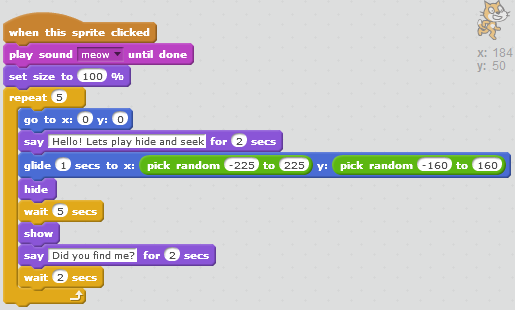
\includegraphics[scale=0.8]{10_ScratchBloks_Version1.png}
	\caption{{10 Scratch Bloks}}
	\label{fig:Version_1.0}
\end{figure}

Changelog:    

\begin{itemize}
	\item Starter med at etablere spritens originalstørrelse.
	\item Gentager sig selv \textbf{5 gange istedet}.
	\item Katten gemmer sig i længere tid.
	\item Katten slutter af med at sige “Did you find me?”
	\item X- og Y-koordinater er nu tilpasset bedre, bl.a. er fladen ikke kvadratisk så Y-aksen skulle tilpasses yderligere.
	\item Fjernede X- og Y-koordinat nulstillingen i slutningen af repeat loopet, da X- og Y-koordinat nulstillingen sker i det første trin der udføres i loopet. 
\end{itemize}


Vi har dog brugt en grøn ‘Vælg tilfældig’-boks\\

Link til programmet: \\
\url{https://scratch.mit.edu/projects/120575598/}



